\section{Extension To Time-Dependent Data}
\label{sec:timeDepRIMs}

In order to extend the calculation presented in Section~\ref{sec:classicalRIMs_RISMC} in the time-domain we need 
additional information: the temporal profile of the status of those components 
that might be taken offline due to maintenance or testing.

We will follow this notation:
\begin{itemize}
  \item $\Xi$ represents the system configuration, i.e.,  the status of components 
              and systems of the plant on the time scale $\tau$ of the plant lifetime
  \item $RAW_i(\tau)$, $FV_i(\tau)$, $RRW_i(\tau))$, $B_i(\tau)$ are the RIMs determined 
        for the basic event $i$ calculated on the time scale $\tau$
\end{itemize}

Note that in our application the status of each component can be only binary: 
component operating or component off-line (i.e., either because it is failed or 
under maintenance/testing). Thus component performance degradation is not considered.
The calculation algorithms is as follows given a set of simulated data:
\begin{enumerate}
  \item Divide the temporal profile into $L$ segments where the status of the components,
        i.e. the system configuration $\Xi$, remain constant
  \item For each time segment, i.e., for $l=1,\ldots,L$ 
        \begin{enumerate}
          \item Determine $R_0$ according to the system configuration $\Xi_l$ for segment $l$
            \begin{equation}
              R_0(l) = \frac{N_{CD, \Xi=\Xi_l}}{N_{\Xi=\Xi_l}} 
              \label{eq:}
            \end{equation}
          \item For each component determine $R_i^-$ and $R_i^+$
          \begin{itemize}
            \item If the component is on-line, $R_i^-$ and $R_i^+$ are determined as follows:
              \begin{equation}
                R_i^+(l) = \frac{N_{CD, s_i \in I_i^+, \Xi=\Xi_l}}{N_{\Xi=\Xi_l}} 
                \label{eq:}
              \end{equation}
              
              \begin{equation}
                R_i^-(l) = \frac{N_{CD, s_i \in I_i^-, \Xi=\Xi_l}}{N_{\Xi=\Xi_l}} 
                \label{eq:}
              \end{equation}
            \item If the component is off-line determine $R_i^+(l)$ according to Eq.~\ref{} and 
                 set $R_i^-(l)=R_i^+(l)$
          \end{itemize}
        \end{enumerate}
\end{enumerate}

\subsection{Test case}
\label{sec:timeDepRIMsExample}

For the scope of this paper we have chosen an example that can help the reader to 
understand the proposed algorithm. This a simple system composed of three components 
(i.e., A, B and C) in a parallel/series configuration shown in Figure~\ref{fig:example12}. 
To each component a failure rate is 
provided when the system is called on demand:
\begin{itemize}
  \item $\lambda_A=1.0 \cdot 10^{-3} hr^{-1}$
  \item $\lambda_B=5.0 \cdot 10^{-3} hr^{-1}$
  \item $\lambda_C=1.0 \cdot 10^{-2} hr^{-1}$
\end{itemize}
  
Even though the system can be solved analytically we have chosen a dynamic method to solve it in 
order to show how the proposed methods is implemented. 
By using a Monte-Carlo based Dynamic PRA method, we have generated a database of simulated data 
where each data point is structured as follows:
\begin{itemize}
  \item Input variables: failure time of components A, B and C (i.e., $s_i$) sampled from their 
        own distribution (i.e., exponential with lambda values provided at the beginning of this section)
  \item Output variables: status of the system (either OK or CD)
\end{itemize}

We have selected the temporal profile for two components: A and C as shown in Fig.~\ref{fig:plotStatus_line-line}. 
By following the algorithm presented above it has been possible to determine the temporal profiles of:
\begin{itemize}
  \item system failure probability (see Fig.~\ref{fig:timeDepPlots} left)
  \item RIMs such as FV (see Fig.~\ref{fig:timeDepPlots} right) 
\end{itemize}

\begin{figure}
    \centering
    \centerline{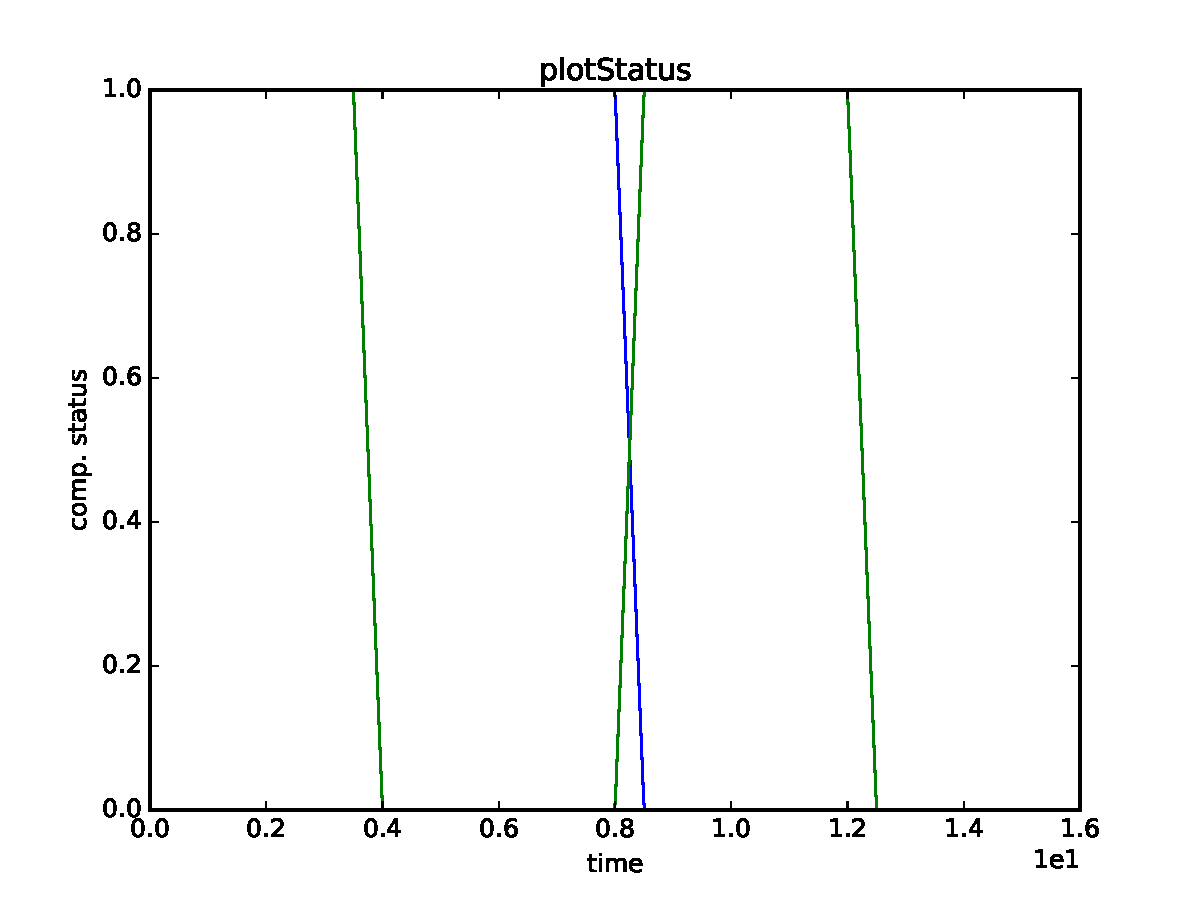
\includegraphics[scale=0.4]{1-plotStatus_line-line.pdf}}
    \caption{Temporal profile of the status for component A (blue line) and C (green line).}
    \label{fig:plotStatus_line-line}
\end{figure}

\begin{figure}
  \centering
  \begin{subfigure}{.5\textwidth}
    \centering
    \centerline{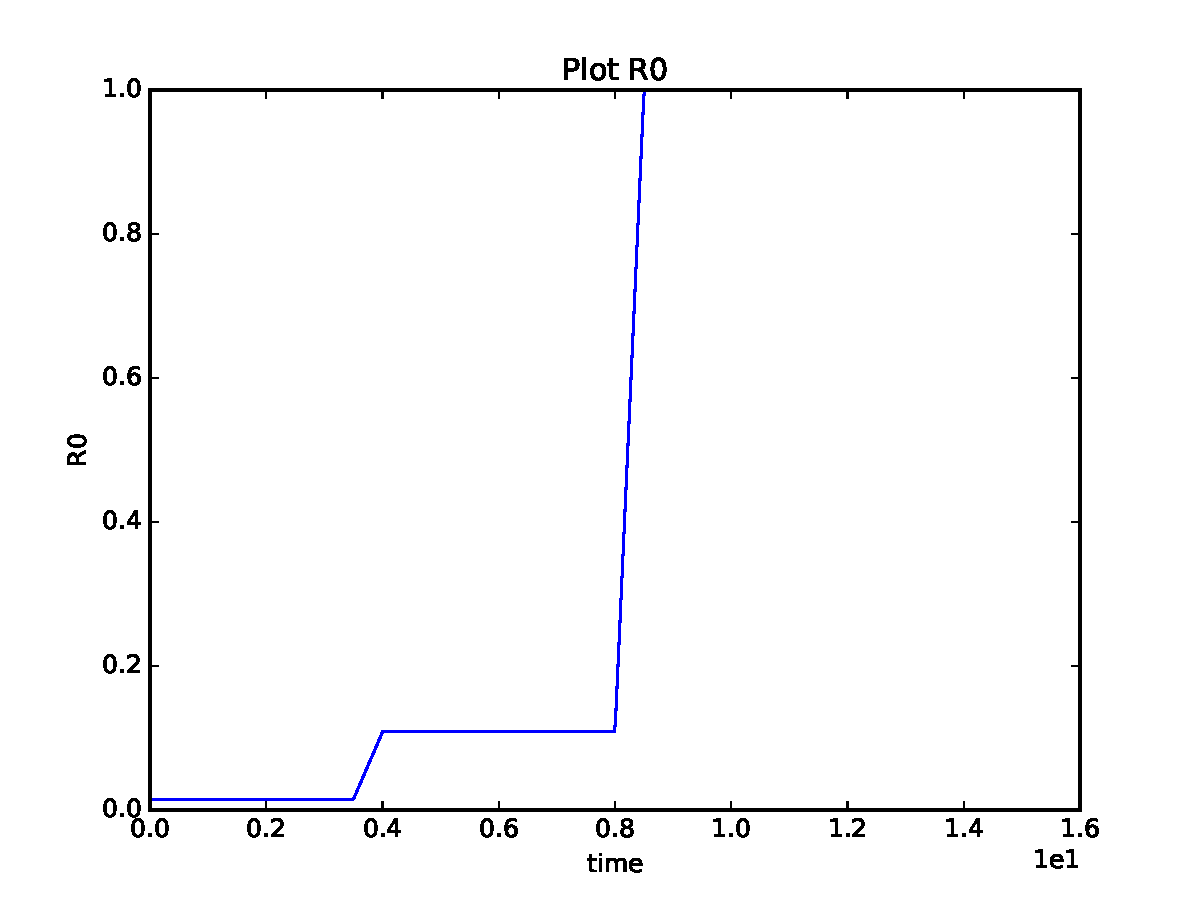
\includegraphics[scale=0.4]{1-plotR0_line.pdf}}
  \end{subfigure}%
  \begin{subfigure}{.5\textwidth}
    \centering
    \centerline{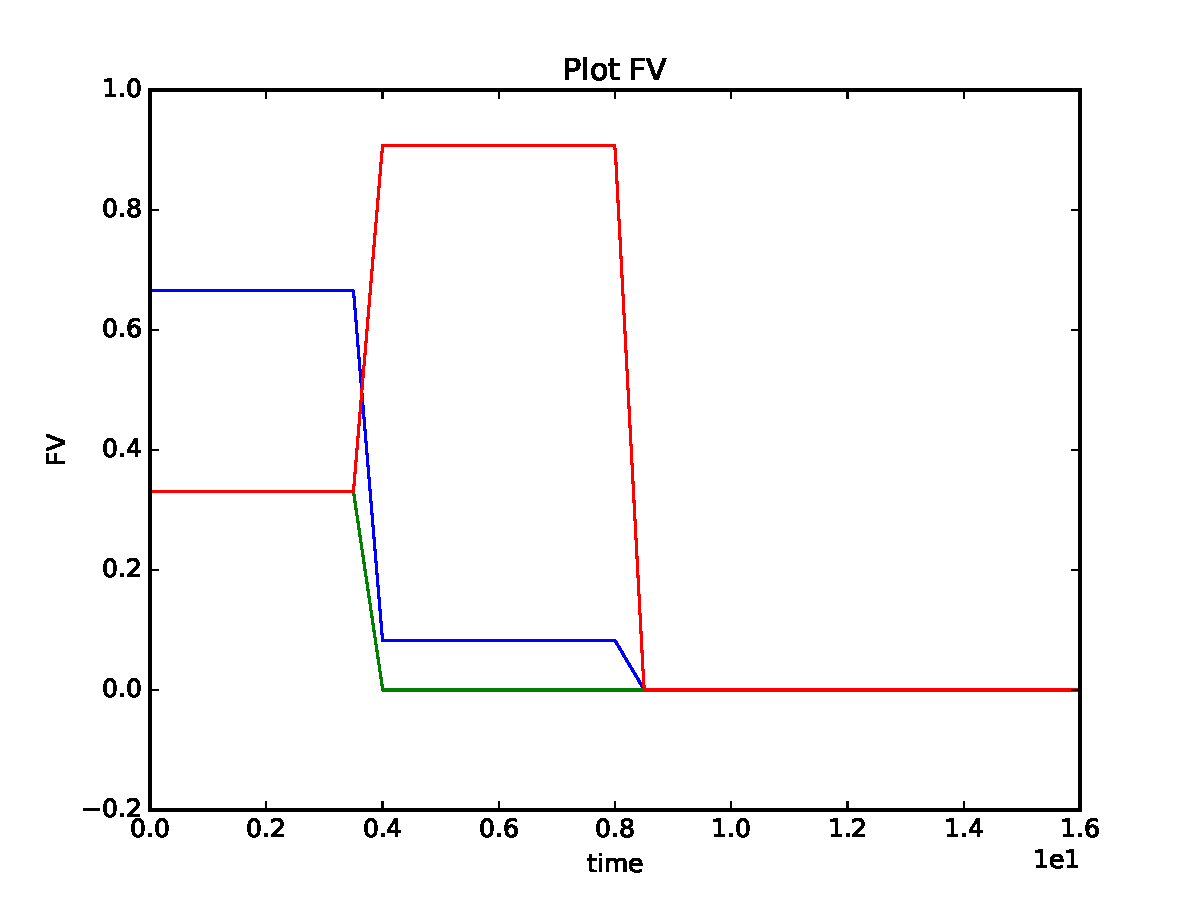
\includegraphics[scale=0.4]{1-plotFV_line-line-line.pdf}}
  \end{subfigure}
  \caption{Temporal profile for system failure probability (left) and FV profile (right) for 
           components B (green line), A (blue line) and C (red line).}
  \label{fig:timeDepPlots}
\end{figure}


